In this section we examine the differences between quark and gluon initiated jets in terms of the substructure variables, and to what extent these variables are correlated. Along the way, we attempt to provide some theoretical understanding of these observations. The motivation for these studies comes not only from the desire to ``tag'' a jet as being quark or gluon initiated, but also from the point of view of understanding the quark and gluon components to the QCD background to boosted boson and boosted top tagging.  

\subsection{Methodology}

%{\it Start adding outline/discussion of theoretical understanding}
These studies use the $qq$ and $gg$ samples, described previously in Section~\ref{sec:samples}.

Jets are reconstructed using the \antikt algorithm, and have various
jet grooming approaches applied, as described in Section~\ref{sec:jetalgs}. The following event selection is then applied to these
samples....(presumably this will vary depending on which kinematic bin
is used, as will the actual samples used - maybe summarize in a table).

Go on to explain how we produce the ROC curves, how the BDT training
is done etc.

Figure~\ref{fig:qg_pt500_basics_AKt_R08} shows a comparison of the quark and gluon samples
in some basic kinematic distributions. 

\begin{figure*}
\begin{center}
\subfigure[Leading jet
\pT]{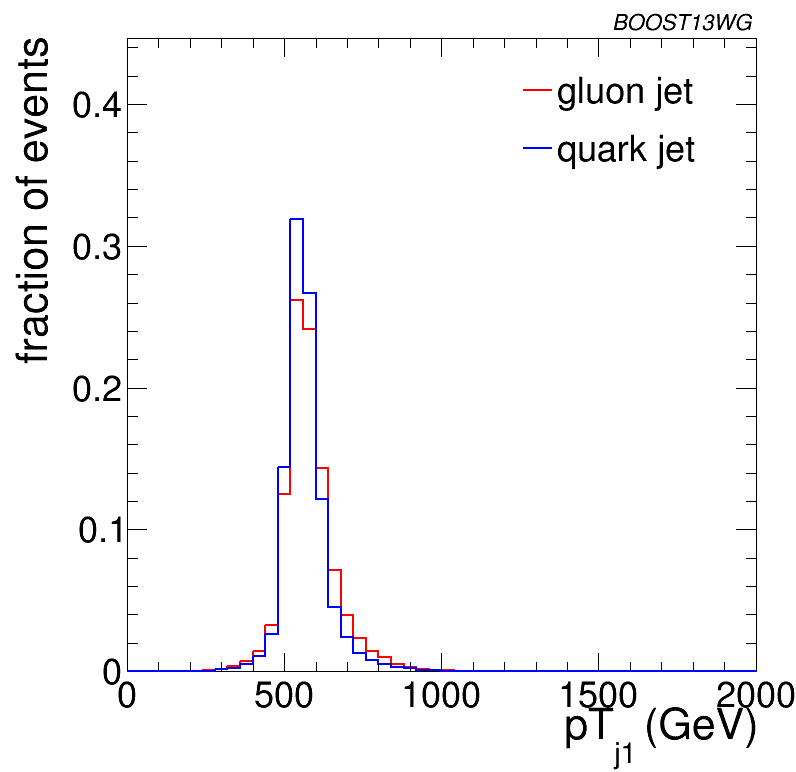
\includegraphics[width=0.40\textwidth]{./Figures/QGTagging/pT500/AKtR08/jpt1.png}}
\subfigure[Sub-leading jet
\pT]{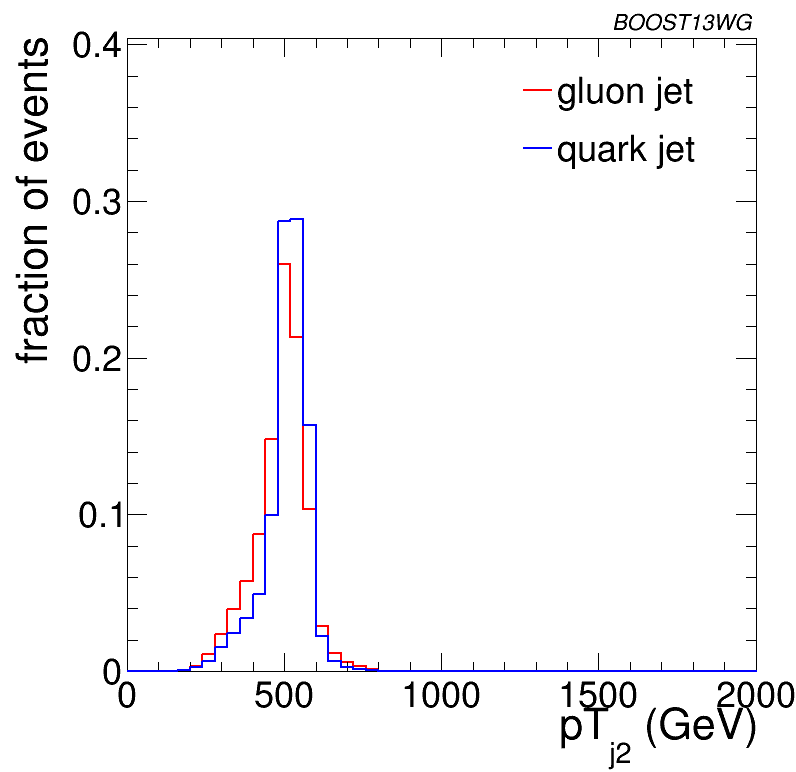
\includegraphics[width=0.40\textwidth]{./Figures/QGTagging/pT500/AKtR08/jpt2.png}}\\
\subfigure[Leading jet
$\eta$]{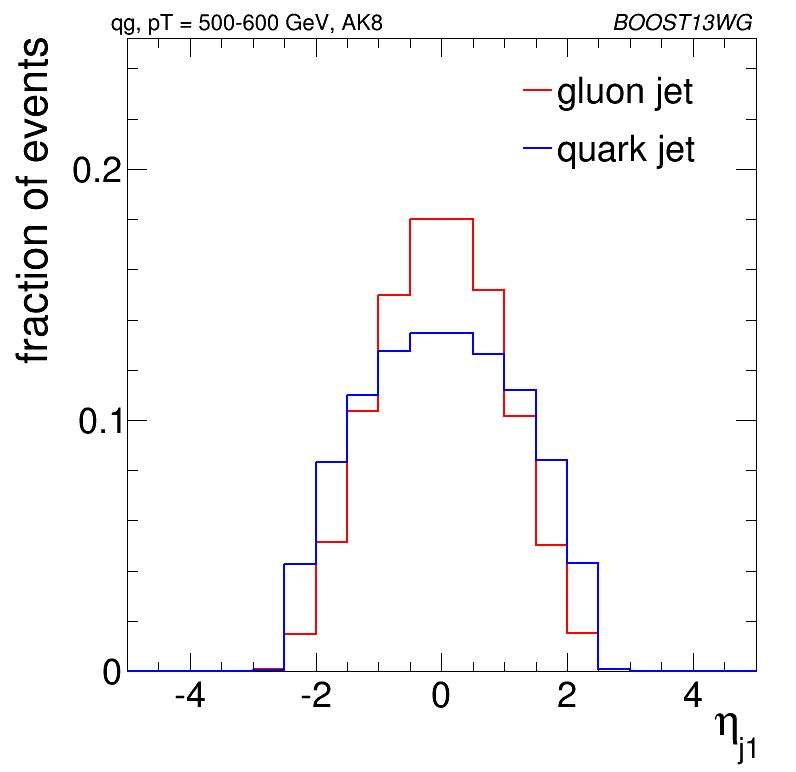
\includegraphics[width=0.40\textwidth]{./Figures/QGTagging/pT500/AKtR08/jeta1.png}}
\subfigure[Sub-leading jet
$\eta$]{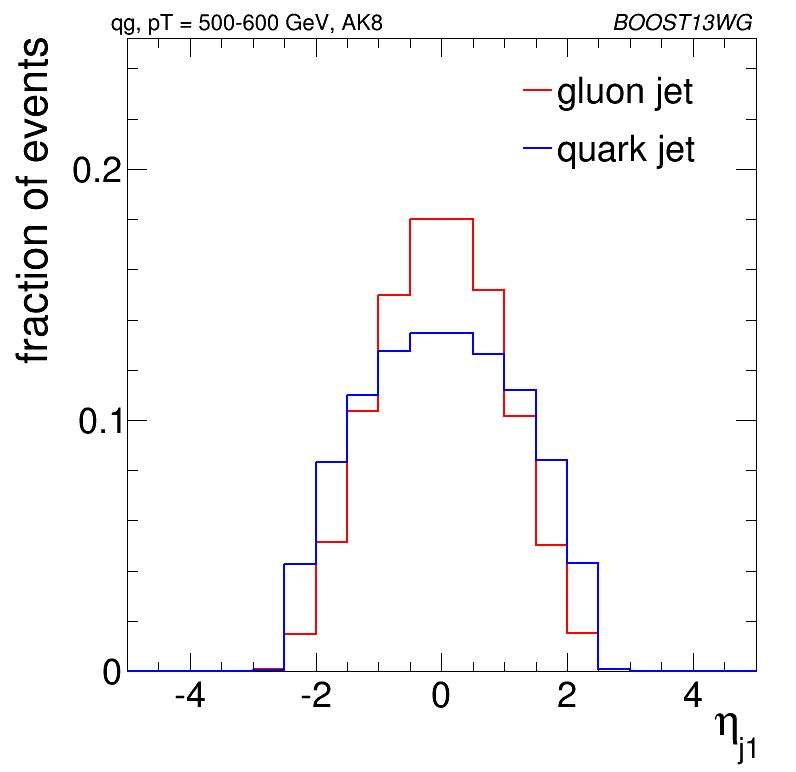
\includegraphics[width=0.40\textwidth]{./Figures/QGTagging/pT500/AKtR08/jeta2.png}}
\caption{Comparisons of quark and gluon distributions in the \pt 500 GeV bin using the anti-\kT R=0.8 algorithm: basic
  kinematic distributons.}
\label{fig:qg_pt500_basics_AKt_R08}
\end{center}
\end{figure*}

\subsection{Single Variable Discrimination}

Figure~\ref{fig:qg_pt500_mass_AKt_R08} the compares the quark and gluon samples
 in the mass distributions for the different groomers, and Figure~\ref{fig:qg_pt500_subst_AKt_R08}
in the different substructure variables. 

\begin{figure*}
\begin{center}
\subfigure[Ungroomed mass]{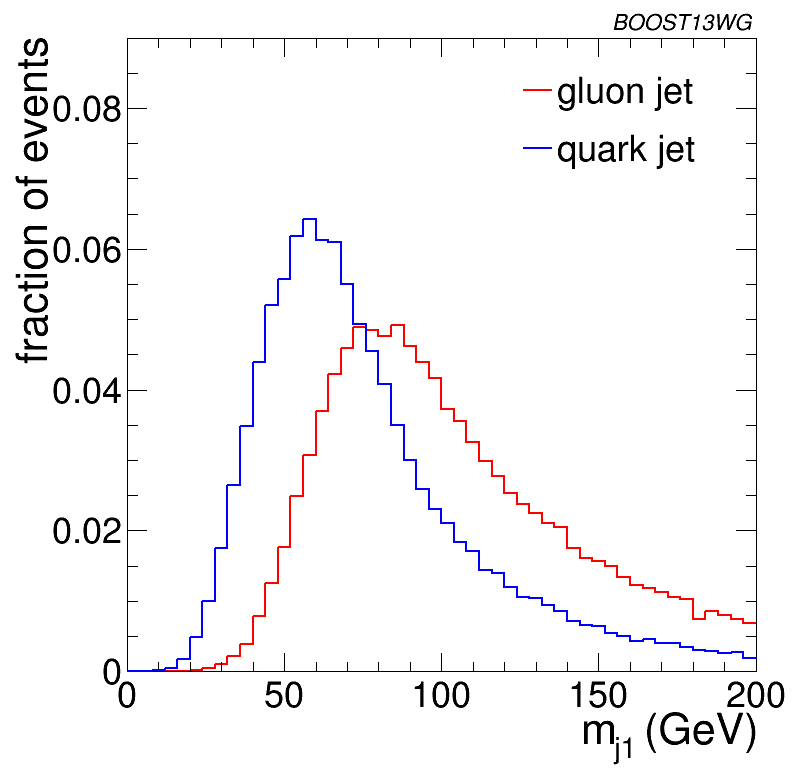
\includegraphics[width=0.30\textwidth]{./Figures/QGTagging/pT500/AKtR08/jmass1.png}}
\subfigure[Pruned mass]{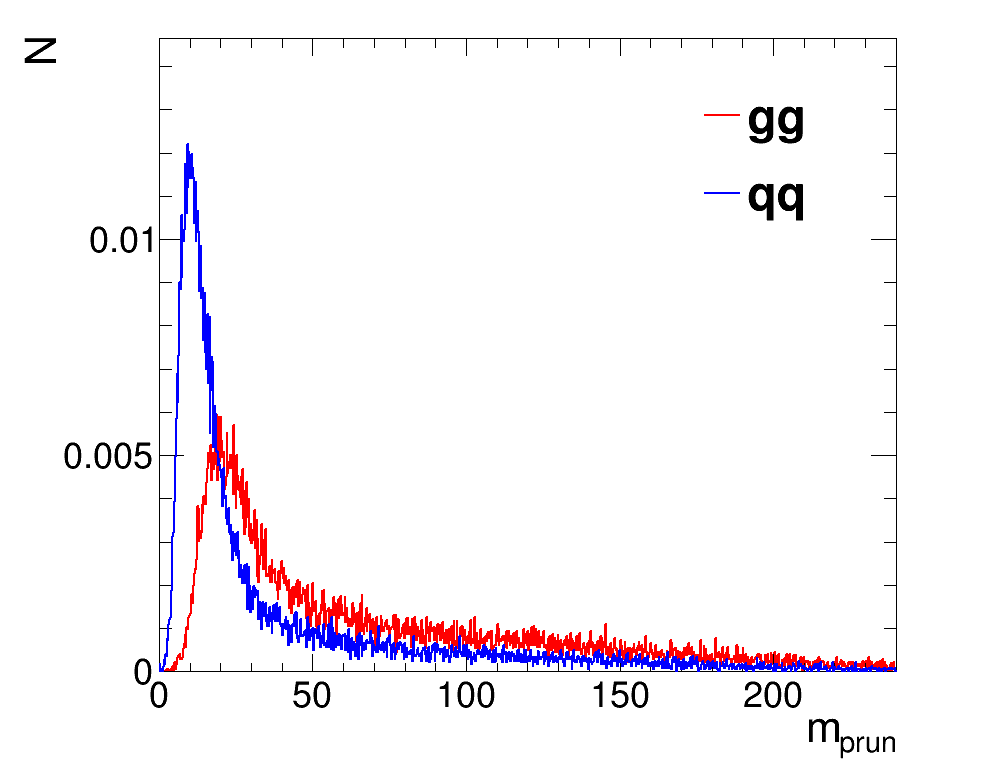
\includegraphics[width=0.30\textwidth]{./Figures/QGTagging/pT500/AKtR08/h_mass_prun.png}}
\subfigure[Trimmed mass]{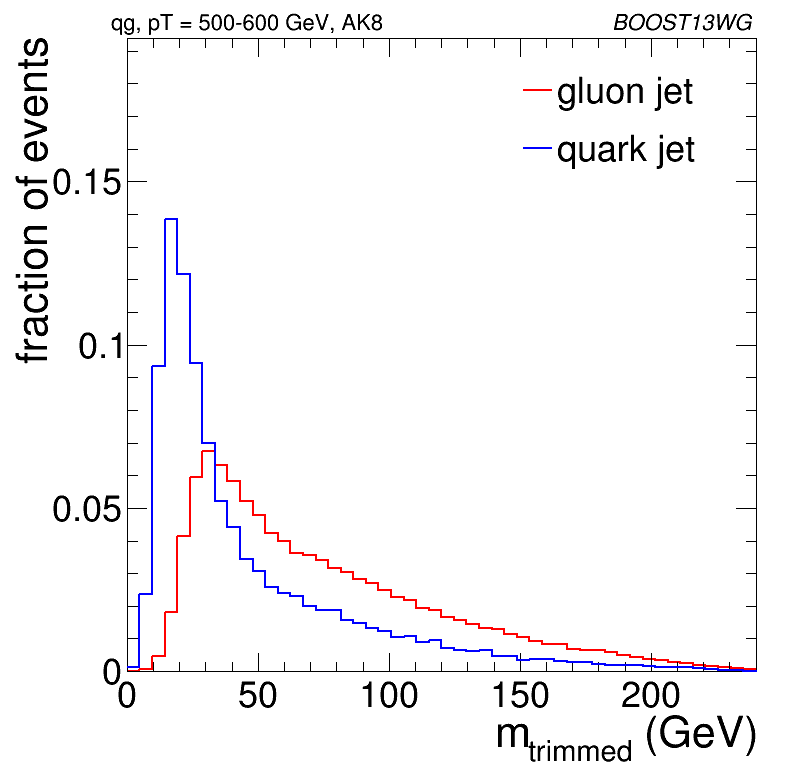
\includegraphics[width=0.30\textwidth]{./Figures/QGTagging/pT500/AKtR08/h_mass_trim.png}}\\
\subfigure[mMDT mass]{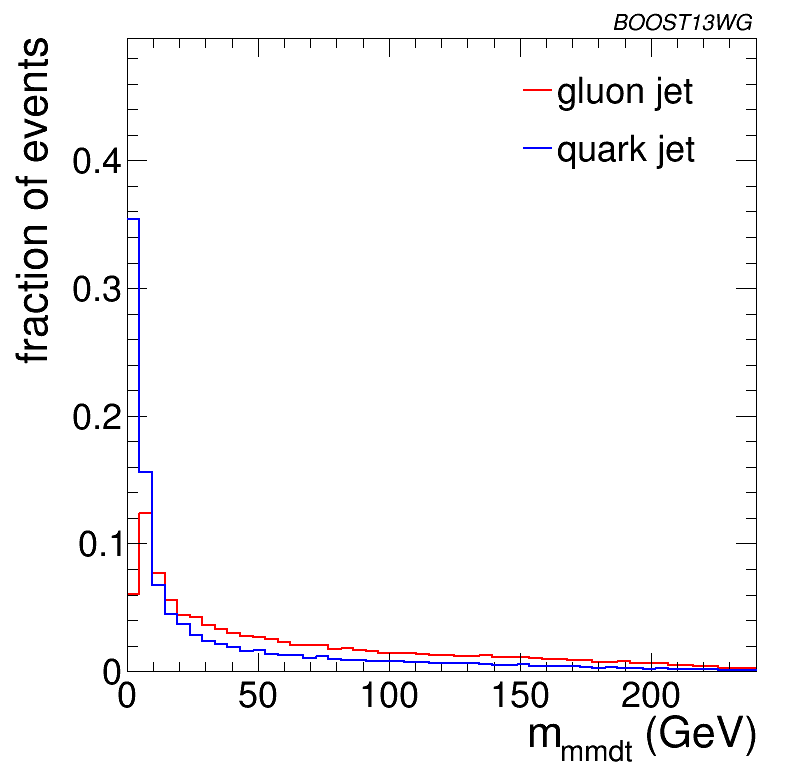
\includegraphics[width=0.30\textwidth]{./Figures/QGTagging/pT500/AKtR08/h_mass_mmdt.png}}
\subfigure[Soft-drop $\beta=2$ mass]{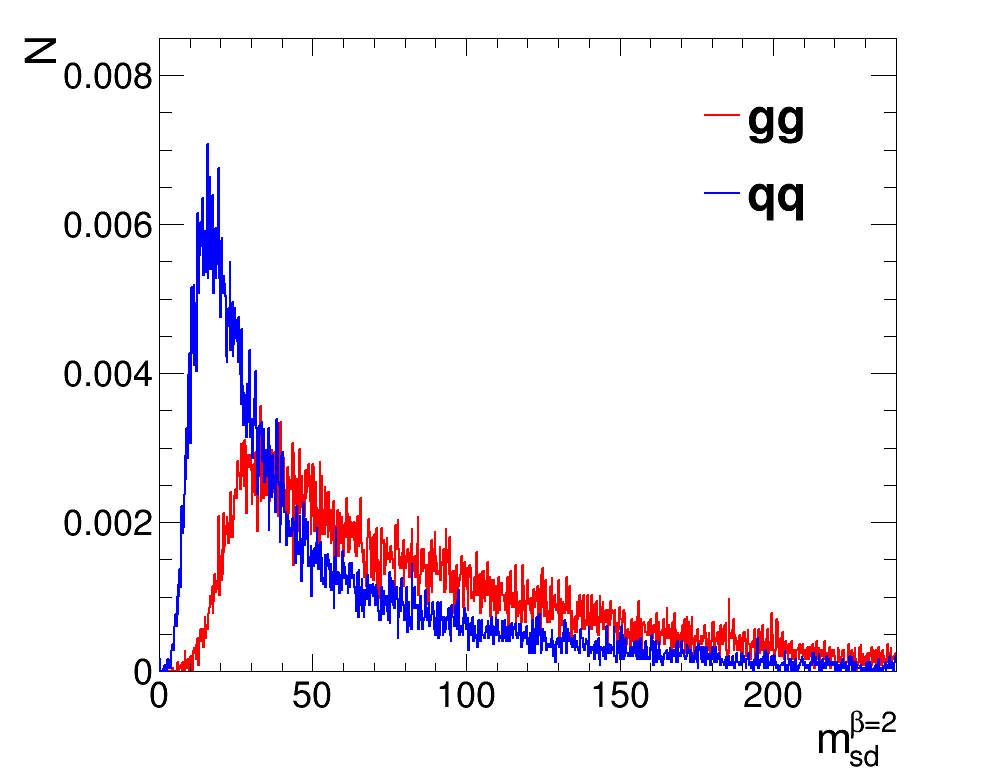
\includegraphics[width=0.30\textwidth]{./Figures/QGTagging/pT500/AKtR08/h_mass_sdb2.png}}
\subfigure[Soft-drop $\beta=-1$ mass]{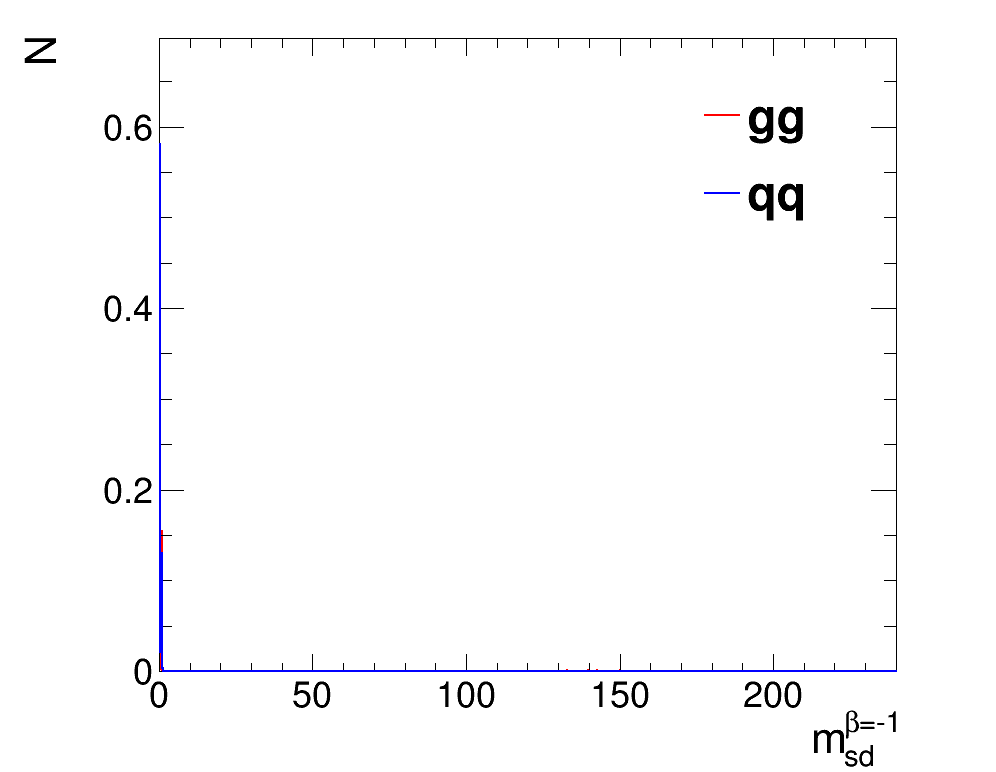
\includegraphics[width=0.30\textwidth]{./Figures/QGTagging/pT500/AKtR08/h_mass_sdm1.png}}
\caption{Comparisons of quark and gluon distributions in the \pt 500 GeV bin using the anti-\kT R=0.8 algorithm: leading
  jet mass distributions.}
\label{fig:qg_pt500_mass_AKt_R08}
\end{center}
\end{figure*}


\begin{figure*}
\begin{center}
\subfigure[$C_1^{\beta=0}$]{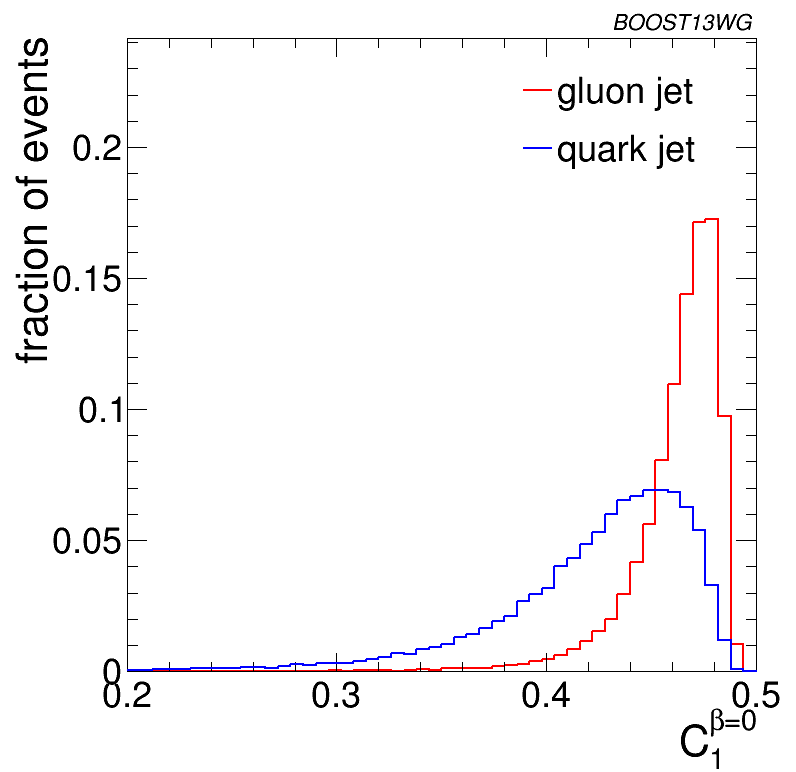
\includegraphics[width=0.30\textwidth]{./Figures/QGTagging/pT500/AKtR08/h_c1_b0.png}}
\subfigure[$C_1^{\beta=1}$]{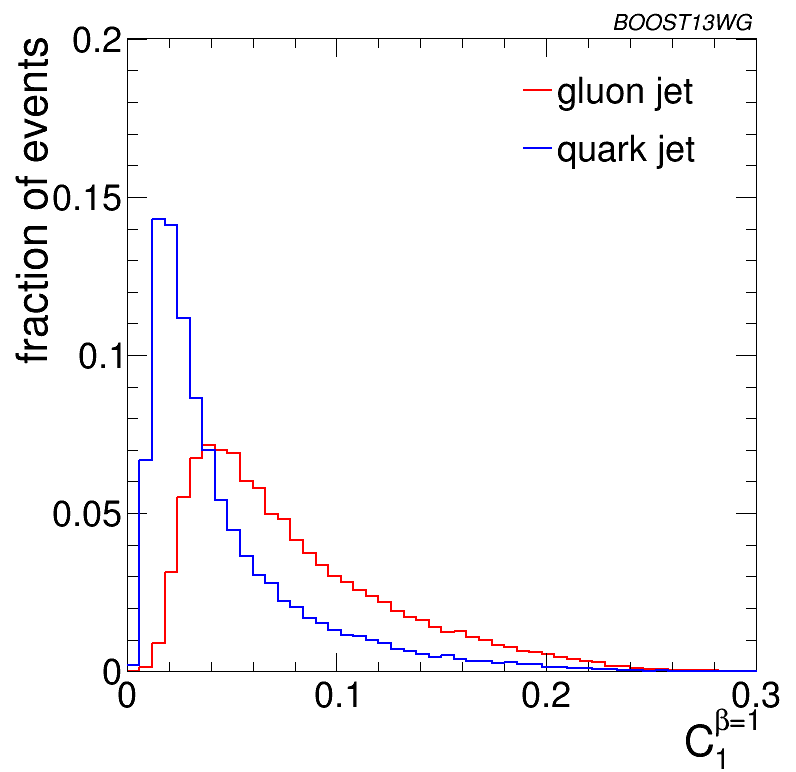
\includegraphics[width=0.30\textwidth]{./Figures/QGTagging/pT500/AKtR08/h_c1_b1.png}}
\subfigure[$C_1^{\beta=2}$]{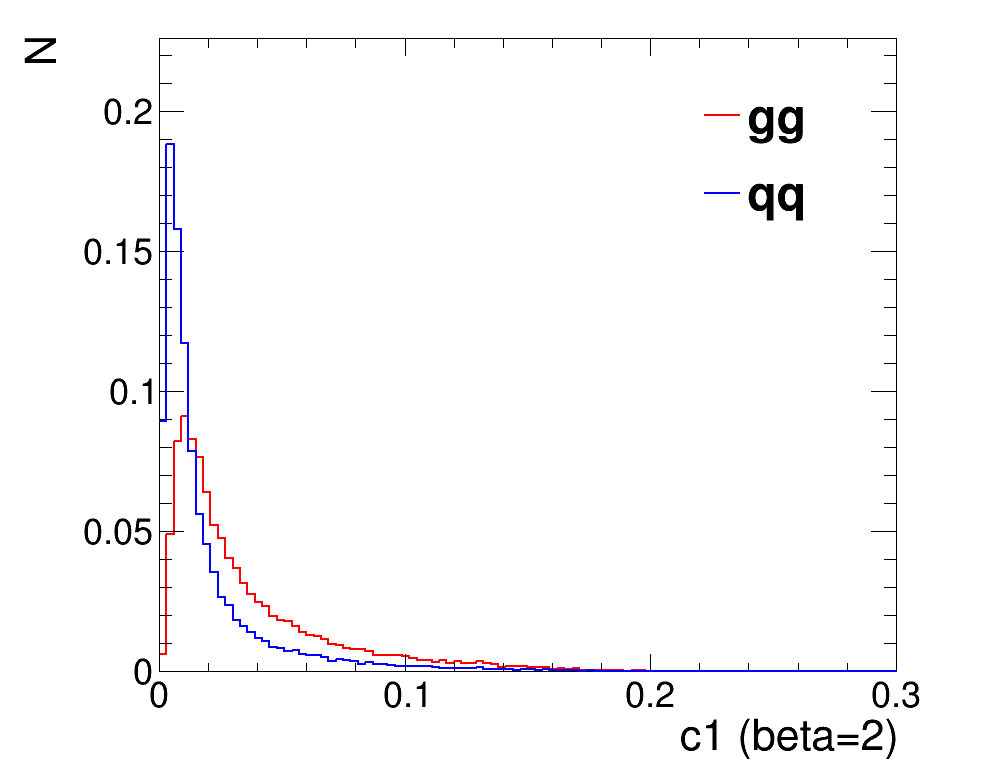
\includegraphics[width=0.30\textwidth]{./Figures/QGTagging/pT500/AKtR08/h_c1_b2.png}}\\
\subfigure[$\Gamma_{Qjet}$]{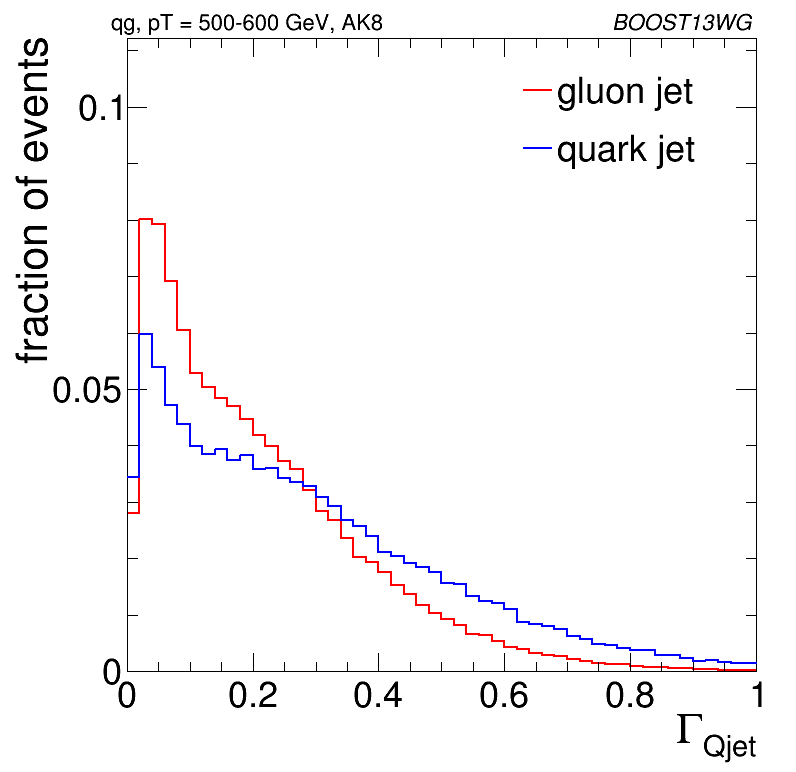
\includegraphics[width=0.30\textwidth]{./Figures/QGTagging/pT500/AKtR08/h_qjetVol.png}}
\subfigure[$\rm{n_ {constits}}$]{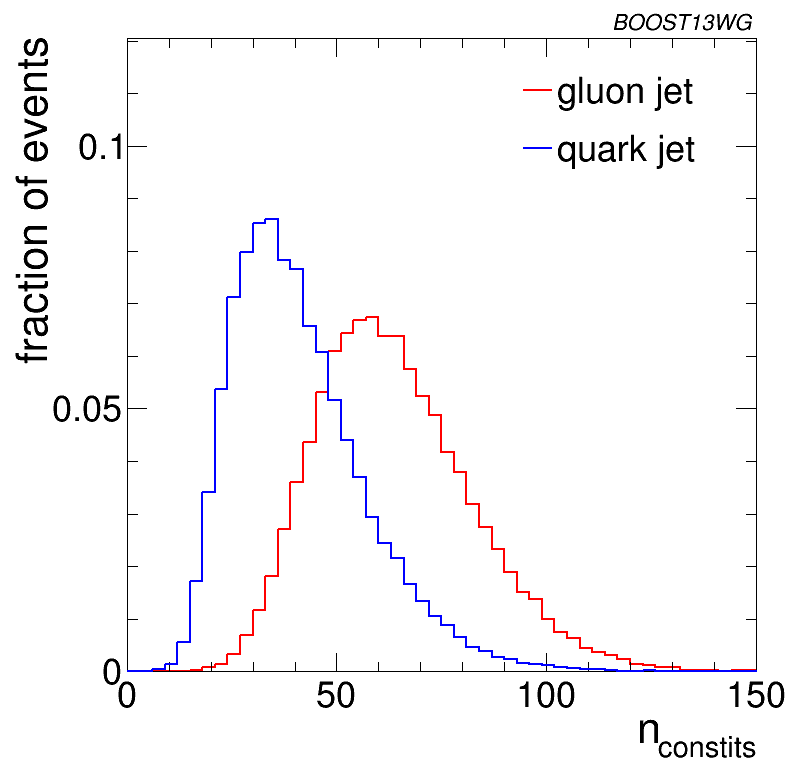
\includegraphics[width=0.30\textwidth]{./Figures/QGTagging/pT500/AKtR08/h_multiplicity.png}}
\subfigure[$\tau_{1}^{\beta=1}$]{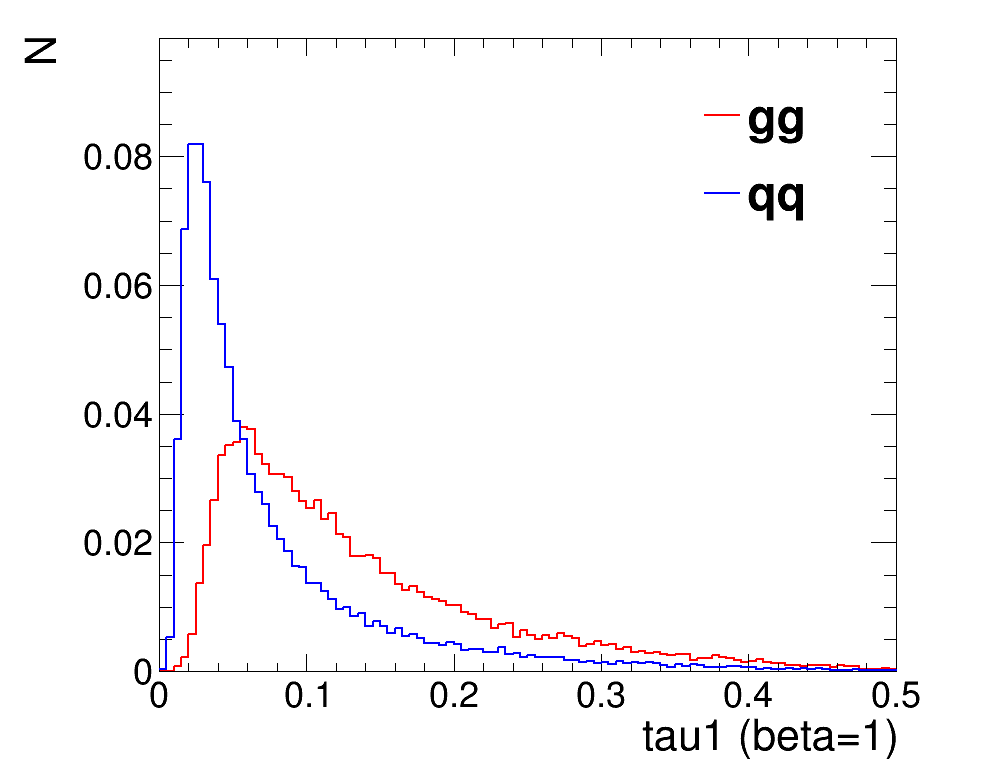
\includegraphics[width=0.30\textwidth]{./Figures/QGTagging/pT500/AKtR08/h_tau1_b1.png}}\\
\subfigure[$\tau_{1}^{\beta=2}$]{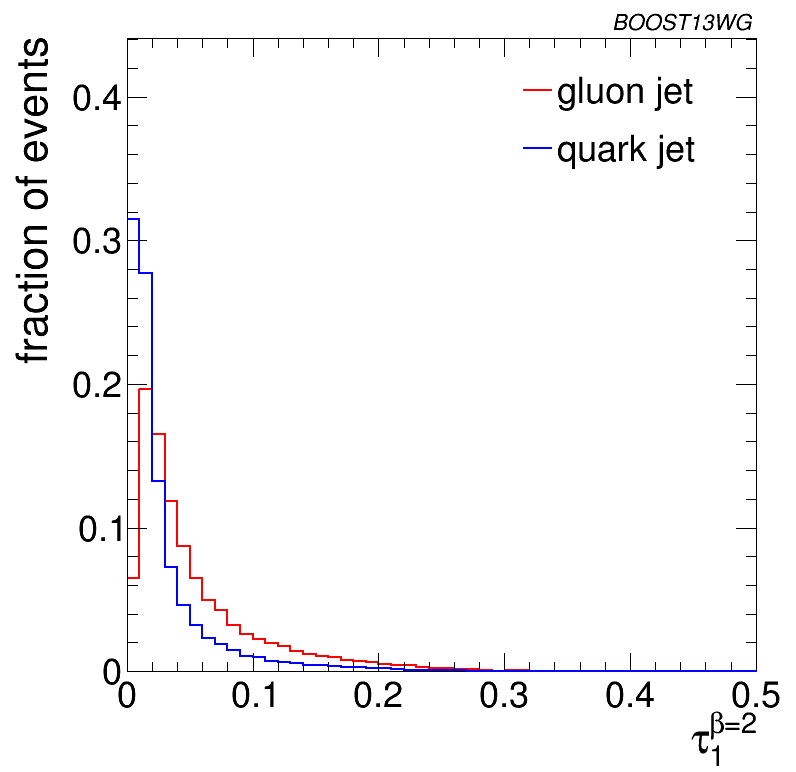
\includegraphics[width=0.30\textwidth]{./Figures/QGTagging/pT500/AKtR08/h_tau1_b2.png}}
\caption{Comparisons of the quark and gluon distributions in the \pt 500 GeV bin using the anti-\kT R=0.8 algorithm:
  substructure variables.}
\label{fig:qg_pt500_subst_AKt_R08}
\end{center}
\end{figure*}

Figure~\ref{fig:qg_pt500_single_AKt_R08} shows the single variable ROC curves in
the \pT 500 GeV bin for the anti-\kT R=0.8 algorithm, compared to the
ROC curve for a BDT combination of all the variables. Only the ungroomed mass is shown. One can see that the single most discriminant variables are $\rm{n_ {constits}}$ and $C_1^{\beta=0}$.

{\it We want to look also at:
\begin{itemize}
\item Dependence on R.
\item Dependence on pT.
\end{itemize}
}

\begin{figure*}
\begin{center}
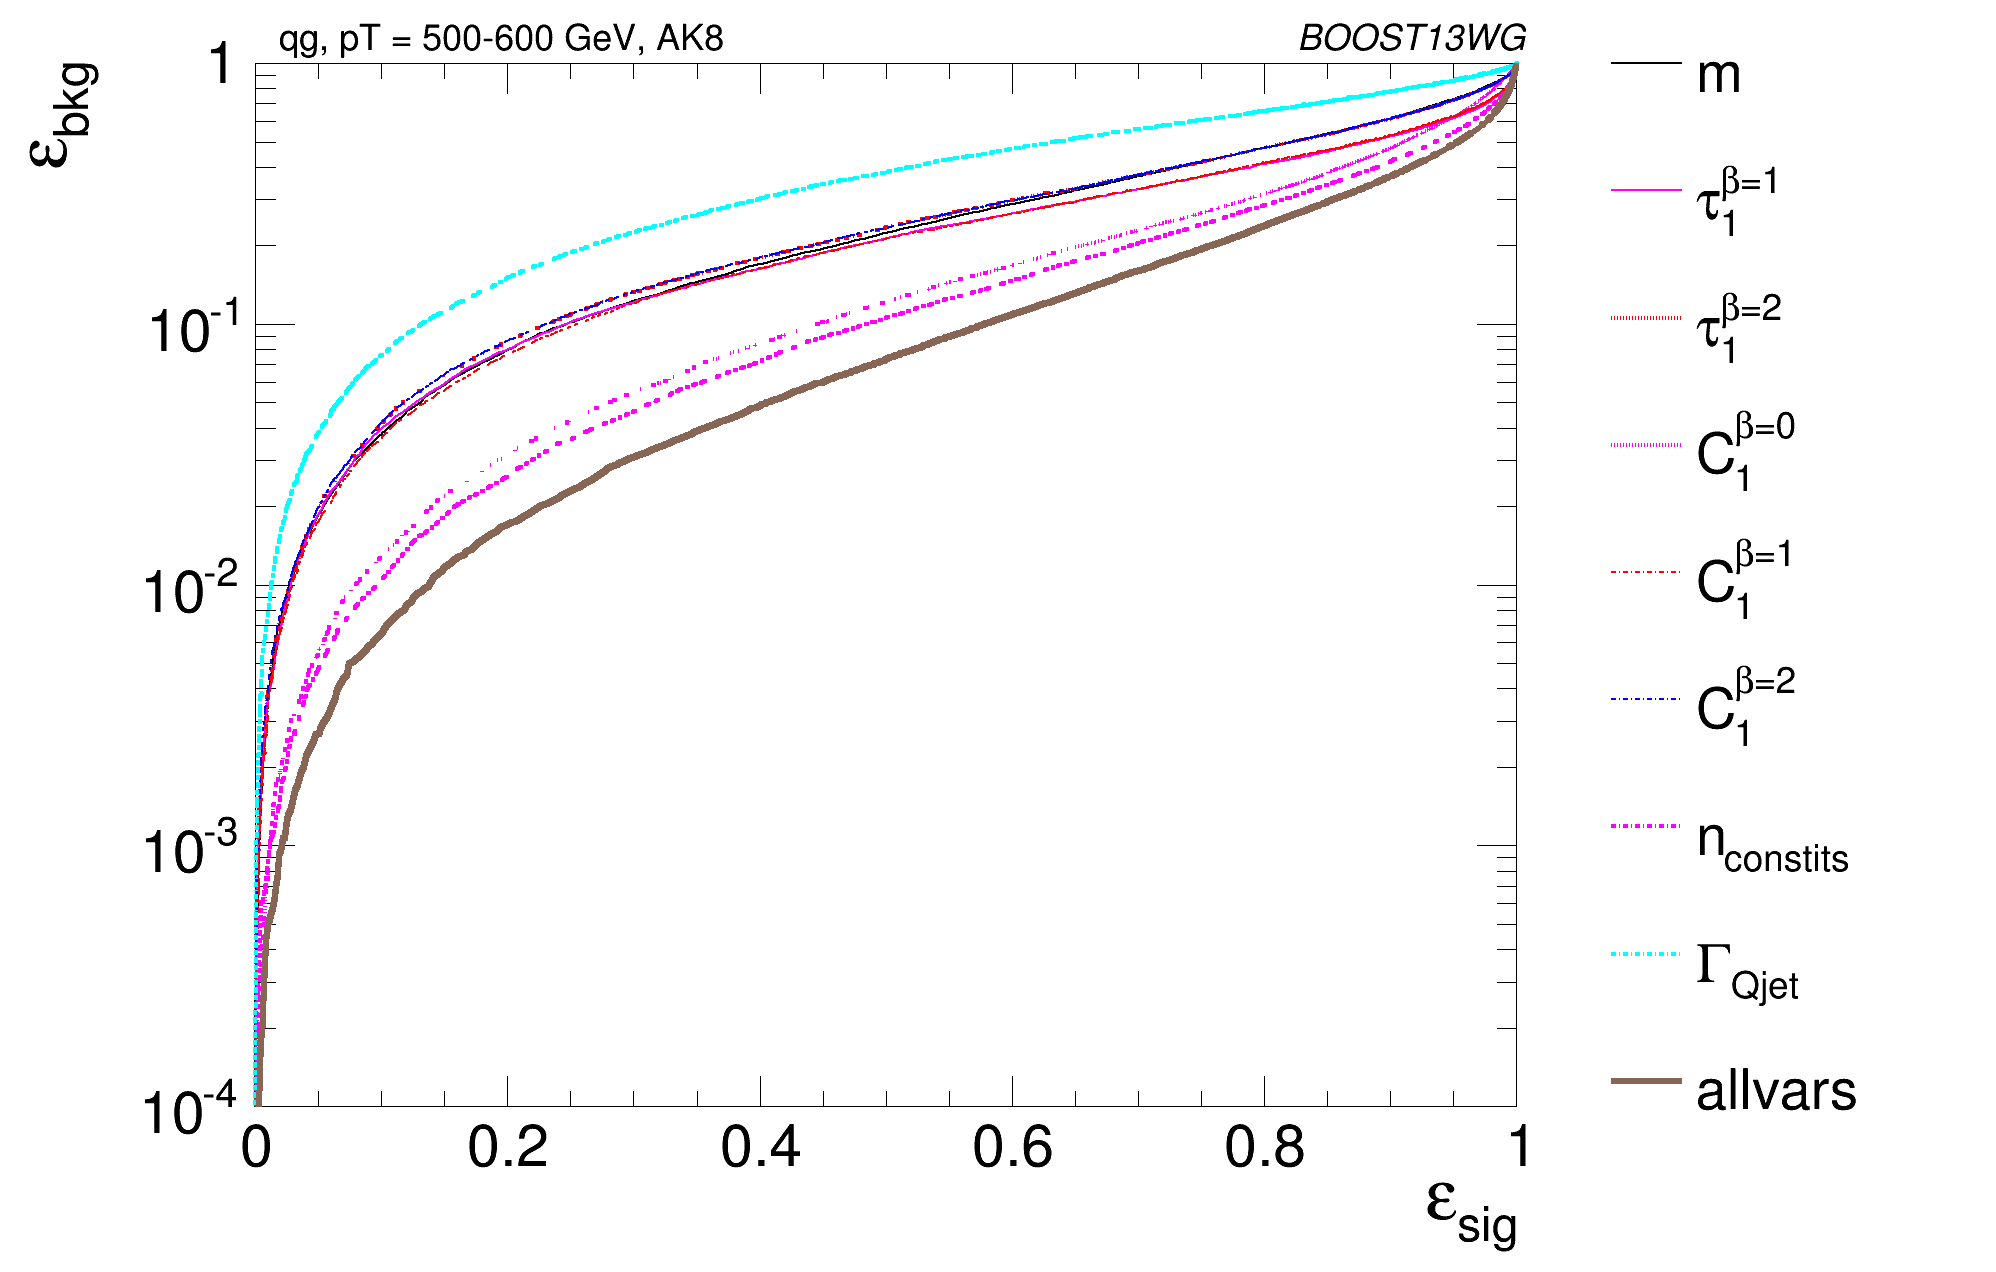
\includegraphics[width=0.8\textwidth]{./Figures/QGTagging/pT500/AKtR08/Rocs_1D_single.png}
\caption{The ROC curve for all single variables considered for quark-gluon discrimination in the \pt 500 GeV bin using the anti-\kT R=0.8 algorithm.}
\label{fig:qg_pt500_single_AKt_R08}
\end{center}
\end{figure*}

\subsection{Correlations}

{\it Put in 2-D plots of correlations between variables (see theory discussions below)}

\subsection{Combined Performance of Quark-Gluon Tagging}

{\it Put in ROC curves of BDT combination of variables}



\subsection{QJets Volatility and $\ptd$ ($\C{1}{\beta=0}$)}

Simple explanation of correlation, or why does combining volatility and $\ptd$ improve quark versus gluon discrimination.  $\ptd$ ($\C{1}{\beta=0}$) takes small (large) values for a jet with near-democratic energy sharing between particles and large (small) values when the energy of the jet is contained in a few particles.  Because we expect gluons to radiate more particles, we expect that $\ptd_g<\ptd_q$ (or ${\C{1}{\beta=0}}_g>{\C{1}{\beta=0}}_q$).  Now, we expect the volatility of gluon jets to be in general smaller than that of quark jets because there is a greater probability (by a factor of about $C_A/C_F=9/4$) that there was a relatively hard emission in a jet that is not groomed away.  By measuring both volatility and $\ptd$, we are sensitive to both regions of phase space: where a relatively hard emission dominates the mass of the jet as well as the region where many soft emissions set the jet mass.

{\it The following is Steve's discussion of volatility difference between quarks and gluons:}

   Here is the (qualitative) thinking:  typical QCD jet mass distributions look as illustrated on slide 17, although you should really be thinking in terms of plot versus $m/p_T$, since $p_T$ is what sets the scale in the plot.  Qualitatively there is a (very) large peak for $m/p_T \lesssim 0.1$ and you should think of these jets as having masses that arise from multiple soft emissions, some of which are at substantial angles.  It is these components of the jet that are operated on by pruning (reducing the mass dramatically) and that yield the large volatility tail for QCD jets.  For larger $m/p_T$ values there is typically a �shoulder� (my description is clearest on a semi-log plot) that runs out to about $m/pT \sim 0.4 � 0.5$ (where the distribution decreases rapidly).  These are the QCD jets (a small fraction of the total in a given $p_T$ bin) that contain a �hard�, relatively large angle emission, which supplies the bulk of the jet mass.  Such jets are effected only slightly by pruning and should exhibit much smaller volatility than the jets in the (smaller mass) peak region.
 
  With that picture in mind and recalling that the size of the �shoulder� is given by low order perturbation theory (the probability of the one hard emission), we expect that the �shoulder� will be higher for gluons than for quarks (essentially by the usual $C_A/C_F$ color charge factor), as suggested by the lower right plot on slide 17.  Since the shoulder presumably plays a more important role for gluons (since it is larger), one would expect that the volatility distribution for gluons is narrower than quarks, as suggested in the upper left plot on slide 17.  Am I making sense?
 
  On the other hand, the volatility distribution plot indicates that the Q vs G distributions for your cuts are not really very different, which is presumably why it is not a very good discriminant by itself.  But I expect this to depend it detail on where we are operating on the m/pT distributions.  This leads to my request above.  Your $p_T$ bin is pretty broad and I don�t expect the q and g samples to have the same shape within the bin.  Of course, this may not be an issue, but I would like to check.


\subsection{Comparison of Groomed Jet Masses}